
%% bare_conf.tex
%% V1.3
%% 2007/01/11
%% by Michael Shell
%% See:
%% http://www.michaelshell.org/
%% for current contact information.
%%
%% This is a skeleton file demonstrating the use of IEEEtran.cls
%% (requires IEEEtran.cls version 1.7 or later) with an IEEE conference paper.
%%
%% Support sites:
%% http://www.michaelshell.org/tex/ieeetran/
%% http://www.ctan.org/tex-archive/macros/latex/contrib/IEEEtran/
%% and
%% http://www.ieee.org/

%%*************************************************************************
%% Legal Notice:
%% This code is offered as-is without any warranty either expressed or
%% implied; without even the implied warranty of MERCHANTABILITY or
%% FITNESS FOR A PARTICULAR PURPOSE! 
%% User assumes all risk.
%% In no event shall IEEE or any contributor to this code be liable for
%% any damages or losses, including, but not limited to, incidental,
%% consequential, or any other damages, resulting from the use or misuse
%% of any information contained here.
%%
%% All comments are the opinions of their respective authors and are not
%% necessarily endorsed by the IEEE.
%%
%% This work is distributed under the LaTeX Project Public License (LPPL)
%% ( http://www.latex-project.org/ ) version 1.3, and may be freely used,
%% distributed and modified. A copy of the LPPL, version 1.3, is included
%% in the base LaTeX documentation of all distributions of LaTeX released
%% 2003/12/01 or later.
%% Retain all contribution notices and credits.
%% ** Modified files should be clearly indicated as such, including  **
%% ** renaming them and changing author support contact information. **
%%
%% File list of work: IEEEtran.cls, IEEEtran_HOWTO.pdf, bare_adv.tex,
%%                    bare_conf.tex, bare_jrnl.tex, bare_jrnl_compsoc.tex
%%*************************************************************************

% *** Authors should verify (and, if needed, correct) their LaTeX system  ***
% *** with the testflow diagnostic prior to trusting their LaTeX platform ***
% *** with production work. IEEE's font choices can trigger bugs that do  ***
% *** not appear when using other class files.                            ***
% The testflow support page is at:
% http://www.michaelshell.org/tex/testflow/



% Note that the a4paper option is mainly intended so that authors in
% countries using A4 can easily print to A4 and see how their papers will
% look in print - the typesetting of the document will not typically be
% affected with changes in paper size (but the bottom and side margins will).
% Use the testflow package mentioned above to verify correct handling of
% both paper sizes by the user's LaTeX system.
%
% Also note that the "draftcls" or "draftclsnofoot", not "draft", option
% should be used if it is desired that the figures are to be displayed in
% draft mode.
%
\documentclass[10pt, conference, compsocconf]{IEEEtran}
% Add the compsocconf option for Computer Society conferences.
%
% If IEEEtran.cls has not been installed into the LaTeX system files,
% manually specify the path to it like:
% \documentclass[conference]{../sty/IEEEtran}

% *** GRAPHICS RELATED PACKAGES ***
%
\usepackage[pdftex]{graphicx}
\graphicspath{{images/}}
\DeclareGraphicsExtensions{.pdf,.jpeg,.png}

% *** MATH PACKAGES ***
\usepackage{amssymb}
\usepackage{amsmath}
\usepackage{xcolor}
\usepackage{url}
\usepackage{algorithm2e}

\newcommand{\todo}[1]{\texttt{\textcolor{red}{#1}}}

% *** ALIGNMENT PACKAGES ***
%
%\usepackage{array}
% Frank Mittelbach's and David Carlisle's array.sty patches and improves
% the standard LaTeX2e array and tabular environments to provide better
% appearance and additional user controls. As the default LaTeX2e table
% generation code is lacking to the point of almost being broken with
% respect to the quality of the end results, all users are strongly
% advised to use an enhanced (at the very least that provided by array.sty)
% set of table tools. array.sty is already installed on most systems. The
% latest version and documentation can be obtained at:
% http://www.ctan.org/tex-archive/macros/latex/required/tools/


%\usepackage{mdwmath}
%\usepackage{mdwtab}
% Also highly recommended is Mark Wooding's extremely powerful MDW tools,
% especially mdwmath.sty and mdwtab.sty which are used to format equations
% and tables, respectively. The MDWtools set is already installed on most
% LaTeX systems. The lastest version and documentation is available at:
% http://www.ctan.org/tex-archive/macros/latex/contrib/mdwtools/


% IEEEtran contains the IEEEeqnarray family of commands that can be used to
% generate multiline equations as well as matrices, tables, etc., of high
% quality.


%\usepackage{eqparbox}
% Also of notable interest is Scott Pakin's eqparbox package for creating
% (automatically sized) equal width boxes - aka "natural width parboxes".
% Available at:
% http://www.ctan.org/tex-archive/macros/latex/contrib/eqparbox/





% *** SUBFIGURE PACKAGES ***
%\usepackage[tight,footnotesize]{subfigure}
% subfigure.sty was written by Steven Douglas Cochran. This package makes it
% easy to put subfigures in your figures. e.g., "Figure 1a and 1b". For IEEE
% work, it is a good idea to load it with the tight package option to reduce
% the amount of white space around the subfigures. subfigure.sty is already
% installed on most LaTeX systems. The latest version and documentation can
% be obtained at:
% http://www.ctan.org/tex-archive/obsolete/macros/latex/contrib/subfigure/
% subfigure.sty has been superceeded by subfig.sty.



%\usepackage[caption=false]{caption}
%\usepackage[font=footnotesize]{subfig}
% subfig.sty, also written by Steven Douglas Cochran, is the modern
% replacement for subfigure.sty. However, subfig.sty requires and
% automatically loads Axel Sommerfeldt's caption.sty which will override
% IEEEtran.cls handling of captions and this will result in nonIEEE style
% figure/table captions. To prevent this problem, be sure and preload
% caption.sty with its "caption=false" package option. This is will preserve
% IEEEtran.cls handing of captions. Version 1.3 (2005/06/28) and later 
% (recommended due to many improvements over 1.2) of subfig.sty supports
% the caption=false option directly:
%\usepackage[caption=false,font=footnotesize]{subfig}
%
% The latest version and documentation can be obtained at:
% http://www.ctan.org/tex-archive/macros/latex/contrib/subfig/
% The latest version and documentation of caption.sty can be obtained at:
% http://www.ctan.org/tex-archive/macros/latex/contrib/caption/




% *** FLOAT PACKAGES ***
%
%\usepackage{fixltx2e}
% fixltx2e, the successor to the earlier fix2col.sty, was written by
% Frank Mittelbach and David Carlisle. This package corrects a few problems
% in the LaTeX2e kernel, the most notable of which is that in current
% LaTeX2e releases, the ordering of single and double column floats is not
% guaranteed to be preserved. Thus, an unpatched LaTeX2e can allow a
% single column figure to be placed prior to an earlier double column
% figure. The latest version and documentation can be found at:
% http://www.ctan.org/tex-archive/macros/latex/base/



%\usepackage{stfloats}
% stfloats.sty was written by Sigitas Tolusis. This package gives LaTeX2e
% the ability to do double column floats at the bottom of the page as well
% as the top. (e.g., "\begin{figure*}[!b]" is not normally possible in
% LaTeX2e). It also provides a command:
%\fnbelowfloat
% to enable the placement of footnotes below bottom floats (the standard
% LaTeX2e kernel puts them above bottom floats). This is an invasive package
% which rewrites many portions of the LaTeX2e float routines. It may not work
% with other packages that modify the LaTeX2e float routines. The latest
% version and documentation can be obtained at:
% http://www.ctan.org/tex-archive/macros/latex/contrib/sttools/
% Documentation is contained in the stfloats.sty comments as well as in the
% presfull.pdf file. Do not use the stfloats baselinefloat ability as IEEE
% does not allow \baselineskip to stretch. Authors submitting work to the
% IEEE should note that IEEE rarely uses double column equations and
% that authors should try to avoid such use. Do not be tempted to use the
% cuted.sty or midfloat.sty packages (also by Sigitas Tolusis) as IEEE does
% not format its papers in such ways.


% *** Do not adjust lengths that control margins, column widths, etc. ***
% *** Do not use packages that alter fonts (such as pslatex).         ***
% There should be no need to do such things with IEEEtran.cls V1.6 and later.
% (Unless specifically asked to do so by the journal or conference you plan
% to submit to, of course. )


% correct bad hyphenation here
\hyphenation{op-tical net-works semi-conduc-tor}


\begin{document}
%
% paper title
% can use linebreaks \\ within to get better formatting as desired
\title{Optimization at Scale with the\\ Alternating Direction Method of Multipliers Algorithm}


% author names and affiliations
% use a multiple column layout for up to two different
% affiliations

\author{\IEEEauthorblockN{Peter Lubell-Doughtie and Jon Sondag}
\IEEEauthorblockA{Intent Media\\
New York, USA\\
\{peter.lubell-doughtie, jon.sondag\}@intentmedia.com}
}

% conference papers do not typically use \thanks and this command
% is locked out in conference mode. If really needed, such as for
% the acknowledgment of grants, issue a \IEEEoverridecommandlockouts
% after \documentclass

% use for special paper notices
%\IEEEspecialpapernotice{(Invited Paper)}




% make the title area
\maketitle


\begin{abstract}
We present a distributed logistic regression algorithm and implementation that performs effectively without parameter tuning.
Although many well known solutions exist, implementing iterative algorithms at scale is a non-trivial exercise.  We implement the Alternating Direction Method of Multipliers (ADMM) algorithm in Apache Hadoop MapReduce and describe how we use the ADMM algorithm to compute logistic regression as a subcomponent in a larger modeling pipeline.  We describe practical lessons learned in implementing an open source ADMM MapReduce algorithm.
\end{abstract}

\begin{IEEEkeywords}
distributed algorithms; optimization; analytics models
\end{IEEEkeywords}


% For peer review papers, you can put extra information on the cover
% page as needed:
% \ifCLASSOPTIONpeerreview
% \begin{center} \bfseries EDICS Category: 3-BBND \end{center}
% \fi
%
% For peerreview papers, this IEEEtran command inserts a page break and
% creates the second title. It will be ignored for other modes.
\IEEEpeerreviewmaketitle



\section{Introduction}
When modeling at scale the solution not only needs to function correctly, it needs to function on large amounts of data in a reasonable amount of time.  In this context, modeling is often approached in a two step process, the first step is to prototype a solution on a sample of the dataset, and the second step is to run it on a production scale dataset.  In many cases production datasets do not fit into the memory available on a single machine and we will need to distribute the dataset over a set of machines.

The MapReduce programming model \cite{dean2004} allows us to work with large distributed data sets.  We use the Apache Hadoop \cite{white2009} implementation of MapReduce which is widely used and supported by many cloud computing providers.  We provide details of implementing an efficient iterative algorithm in Hadoop and how to overcome the challenges of network latency when transferring large amounts of data between clusters in the Amazon ecosystem. 

When using distributed datasets we must use algorithms which can compute on distributed datasets.  The ADMM algorithm is a distributed convex optimization algorithm that allows us to fit logistic regression, lasso, $\ell1$ and $\ell2$ norm, support vector machine, and other popular models.  We can use without having to hand-tune parameters, which is especially time-consuming with long-running modeling jobs.

The model that we prototyped predicted the estimated value $\hat{y}$ as the expectation of the target value $b$ given that this target value is greater than zero and there is a matrix of features $\mathbf{A}$, multiplied by the probability that the target is greater than zero given the features.  We express this as:
\begin{equation}
\hat{y} = \mathbb{E}[b|b>0,\mathbf{A}]P(b>0|\mathbf{A}),
\end{equation}
where we fit the expectation, $\mathbb{E}[b|b>0,\mathbf{A}]$, using linear regression and we fit the conditional probability, $P(b>0|\mathbf{A})$, using logistic regression.  This model performed quite well in prototyping, and the next step was to test it on a production scale dataset.  Fitting linear regression is simple and we use matrix algebra to compute an analytic solution.  However, there is no analytic solution for logistic regression.

To fit the logistic regression model we must use an approximate method.  Many of the approximate methods traditionally used to fit logistic regression require access to the entire training dataset at once, i.e. they require that the training data set can be fit into memory and because of this they cannot be distributed.  However, the ADMM algorithm does not have this property.

The ADMM algorithm is an optimization algorithm suitable for convex optimization which can be used to compute logistic regression on subdivided portions of the training data and then combine the calculations on each portion to find a global solution \cite{boyd}.  Because of this the ADMM algorithm is amenable to the MapReduce programming model which distributes computations to multiple nodes.  On each iteration the ADMM algorithm optimizes the objective function for each portion of training data, it then aggregates these predictions to find the global solution.

The rest of the paper is organized as follows.  In section \ref{sec:imp} we provide details concerning our implementation of the ADMM algorithm, its application to logistic regression, and how to implement it in Hadoop MapReduce.  In section \ref{sec:results} we present the results of running ADMM on a production scale datasets including the improvement in the objective function and the computation time taken per iteration.  In section \ref{sec:related} we review recent work related to iterative optimization with Hadoop, and in section \ref{sec:conc} we conclude and mention future work.

\section{Implementation}\label{sec:imp}
Here we describe exactly how we implemented ADMM for Hadoop MapReduce and provide practical details relevant to using it to build models in a production environment.

\begin{figure}[!t]
\centering
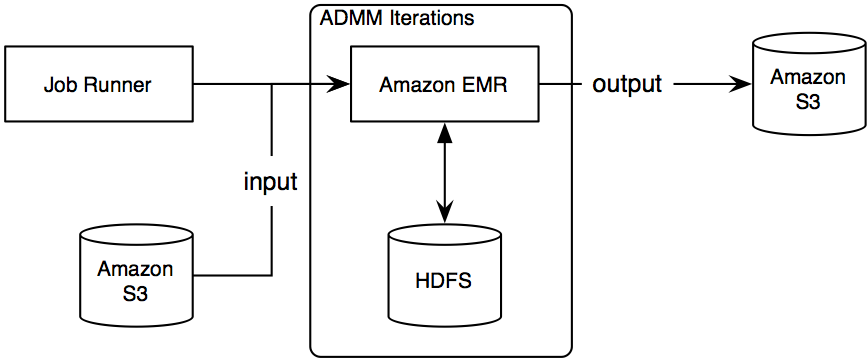
\includegraphics[width=3.2in]{aws_implementation}
\caption{The Job Runner sets paths for the input, the output data, the Jar file with ADMM, and any adjustable parameters; e.g. the number of iterations.  ADMM computes and stores intermediate data in HDFS, then after the final iteration, the $\hat{y}$ values are output to S3.}
\label{workflow}
\end{figure}

\subsection{Logistic Regression with ADMM}
Given a matrix of features $A\in\mathbf{R}^{n\times m}$ and a vector of their labels $b\in\{-1,1\}$, our goal is to compute the probability $\text{Pr}(B_i=b_i|\mathbf{A}_i)$ for each row $0<i\leq n$.

To compute this probability we fit a logistic regression model using ADMM.  We begin by expressing the logistic regression problem in ADMM form as:
\begin{align*}
\text{minimize}&\quad (1/2)\|Ax-b\|_2^2+\lambda\|z\|_1\\
\text{subject to}&\quad Fx-z=0,
\end{align*}
where we have introduced the regularization factor $\lambda$, as well as the $x$ and $z$ variables.

Given this form we construct the ADMM algorithm:
\begin{align}
\label{eq:x}
x_i^{k+1} :=&\quad \min_{x_i} \sum_{j=1}^Nl(A_{ij}x_i\times b_{ij}) + \dfrac{\rho^k}{2}\|x_i - z^k + u_i^k\|_2^2\\
\label{eq:z}
z^{k+1} :=&\quad \begin{cases}
    x_0^{k+1} + u_0^k& \text{if $i=0$}\\
    \\
    \dfrac{m}{2\lambda}(x_i^{k+1} + u_i^k)& \text{otherwise}
  \end{cases}\\
\nonumber\\
\label{eq:u}
u_i^{k+1} :=&\quad u_i^k + x_i^{k+1} + z^{k+1},
\end{align}
where $l$ is the logistic loss function with $\ell1$ regularization,
\begin{equation*}
l(\alpha)=\log(1+\exp(-\alpha)),
\end{equation*}
$m$ is the number of mappers (explained below), and $\rho^k$ is the penalty parameter for iteration $k$, which is used as the step size.

To solve the minimization function in the $x_i$ update we use the quasi-Newton method of Broyden, Fletcher, Goldfarb, and Shanno---the BFGS method \cite{bonnans2003numerical}.  BFGS is a hill-climbing algorithm that approximates Newton's method and has proven good performance even for non-smooth functions.  We use a Java implementation of BFGS which is self contained and has performed well on Hadoop nodes.\footnote{\url{https://code.google.com/p/vladium/}}

\subsection{ADMM within MapReduce}
The MapReduce model divides into three phases: the map, the shuffle, and the reduce.  In the mapper phase the input data is split among a set of mappers and each mapper applies a function to the set of data assigned to it.  In the shuffle phase the output of the mappers is assigned to a reducer, and then in the reduce phase the mapper output is aggregated to create the final values.

We may express the map and reduce steps the as:
\begin{alignat*}{2}
&\text{map}\quad &(k_1,v_2)\quad\rightarrow &\texttt{list}(k_2,v_2)\\
&\text{reduce}\quad &(k_2,\texttt{list}(v_2))\quad\rightarrow &\texttt{list}(v_2),
\end{alignat*}
where each mapper has a unique key $k_1$.  The shuffle is concerned with mapping the intermediate key-value pairs, $(k_2,v_2)$, otuput by the mappers to the reducers \cite{dean2004}.

To implement MapReduce in Hadoop we must define classes for the mapper, reducer, and a driver that handles input arguments and coordinates the execution of the mapper and reducer (the shuffle is handled by Hadoop).  In the context of ADMM each mapper performs the resource intensive task of computing the current $x_i$.  After all mappers have completed their computations, we use a single reducer to compute the $z_i$ and $u_i$ updates.

\subsubsection{Peristent Data with Input Splits}
In the ADMM algorithm, when each mapper calculates the $x_i^{k+1}$ values on iteration $k+1$, it must use the $u_i^k$ values that were calculated for the same mapper in the previous iteration $k$.  Hadoop does not normally accommodate this sort of persistence.  \cite{boyd} suggest using Apache HBase, a distributed data store, however this would add a new component and its accompanying complexity to the modeling framework.

As an alternative, we use Hadoop's notion of input splits to keep track of where data is stored and associated the correct $x_i$ and $u_i$ values with each other.  Input splits specify a \em{split length} and a \em{split ID}, which determine the size of the split data and the node on which to execute the split, respectively.  To ensure that the correct $u_i$ values are loaded when calculating an $x_i$ value, the mapper reads the split ID and chooses the $u_i$ values based on this split ID.  The $z$ values are the same in each $x_i$ formula, i.e. across mappers, to handle this we simply replicate the current $z$ values across all mappers at the start of each iteration.

\subsubsection{Automatically Updating $\rho$}

We use the reducer to update the penalty parameter $\rho$.  The number of iterations before convergence depends upon the $\rho$ parameter, and hand-tuning the $\rho$ parameter can take a significant amount of time.  We must wait for the algorithm to complete before determining the efficacy of the chosen $\rho$.  By varying the penalty parameter we can reduce the performance impact of our initial choice of $\rho$, and avoid spending time hand-tuning $\rho$.  We use the update scheme suggested in \cite{boyd} to update $\rho$ on each iteration:
\begin{equation}
\rho^{k+1}:=\begin{cases}
  \tau^{\text{incr}}\rho^k&\quad \text{if $\|r^k\|_2>\mu\|s^k\|_2$}\\
  \rho^k/\tau^{\text{decr}}&\quad \text{if $\|s^k\|_2>\mu\|r^k\|_2$}\\
  \rho^k&\quad \text{otherwise,}
\end{cases}
\label{eq:r}
\end{equation}
where $\mu>1$, $\tau^{\text{incr}}>1$, and $\tau^{\text{decr}}>1$ are parameters.  We have used the typical values of $\mu=10$ and $\tau^{\text{incr}}=\tau^{\text{decr}}=2$.

\subsubsection{ADMM Algorithm for MapReduce}
After having completed a mapper and reducer cycle, we will have one iteration of the algorithm has finished and control returns to the driver.  In addition to initiating the mapper and reducer tasks, the ADMM driver determines if the algorithm has converged.  If it has not converged we distribute the $z$ and $u_i$ to the mappers and begin the next iteration, if it has converged we write the results to persistent storage (a bucket on Amazon S3) and exit.  This is shown in Algorithm \ref{alg:admm} below.

\begin{algorithm}
\SetAlgoLined
\KwData{feature matrix $\mathbf{A}$ and vector of target values $b$}
\KwResult{a vector of weights $z$}
$k=0$\\
$m=\text{[the number of mapper nodes]}$\\
\While{$k<\text{maxIterations}$ and $\text{curSt} > \text{preSt}$}{
  \For{$i=1\to m$}{
    update $x_i^k$ using Eq. \ref{eq:x}\\
   update $u_i^k$ using Eq. \ref{eq:u}\\
    $i \gets i + 1$
  }
  update $z^k$ using Eq. \ref{eq:z}\\
  update $\rho^k$ using Eq. \ref{eq:r}\\
  $k \gets k + 1$
}
write $z^k$ to S3.
\label{alg:admm}
\vspace{1em}
\caption{ADMM algorithm implemented for Hadoop MapReduce.}
\end{algorithm}

The data that is used in the algorithm is stored in Amazon's simple storage service, Amazon S3.  To reduce the network latency involved in transferring data from Amazon S3 to MapReduce nodes, we store the data---feature matrix $\mathbf{A}$ and target values $b$---in the nodes' local HDFS file systems.  We use Amazon's Elastic Map Reduce (EMR) service to execute Hadoop, this allows us to avoid any data transfer fees.

Wherever feasible we have made the implementation of the ADMM algorithm generic.  Arguments to the driver allow users to exclude columns from the input data, add an intercept, set the initial $\rho$, maximum number of iterations, and the input and output locations. We have released an implementation of the ADMM algorithm for Hadoop as an open source Java package.\footnote{\url{https://github.com/intentmedia/admm}}.

\section{Results}\label{sec:results}
We run the ADMM algorithm daily on nearly a terabyte of data.  To evaluate the performance we will examine the iterative output of one day's run.  Figure \ref{fig:iter} shows the difference between the predicted function and the actual function per iteration in the left panel, and the time per iteration in the right panel.  We see that the accuracy consistently improves and the run-time consistently decreases for later iterations.

\begin{figure}[!t]
\centering
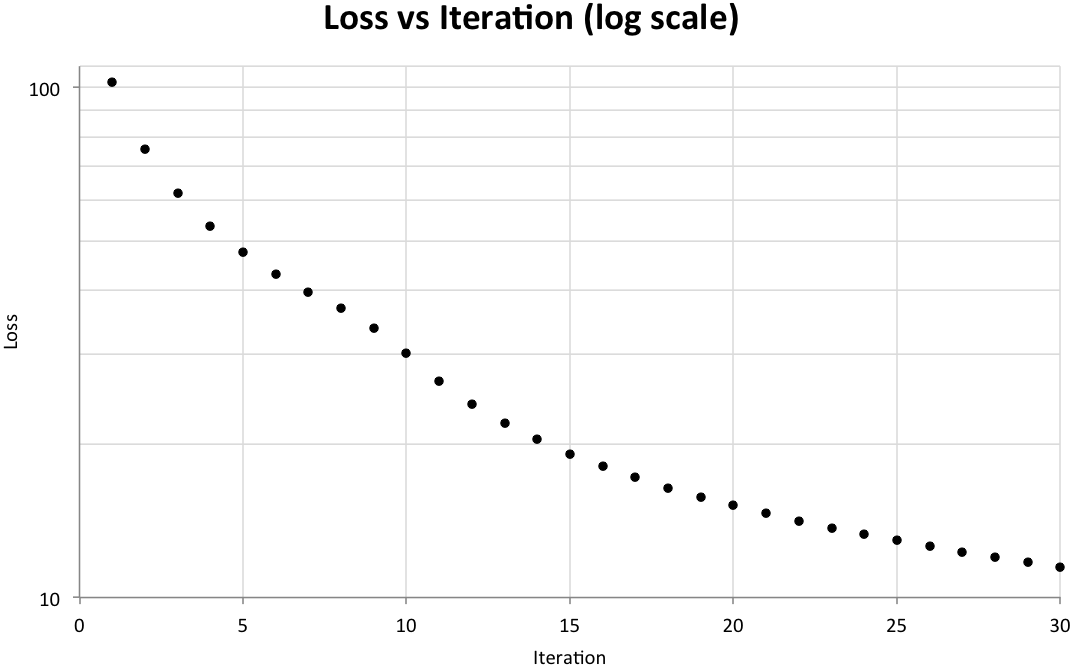
\includegraphics[width=3.2in]{iter_rnorm_plot}
\caption{Loss between our models predictions and the actual values per iteration on a logarithmic scale.  We see that the loss decreases dramatically and then decelerates at later iterations.}
\label{fig:iter}
\end{figure}

\section{Related Work}\label{sec:related}
The algorithm and our implementation are based upon \cite{boyd}, which introduced the ADMM algorithm.  \cite{bu2010} presents a more efficient approach to iterative computation in Hadoop with modifications to the core Hadoop that reduce the costs of transferring data.  This is not the approach we took, we decided to stay within the Hadoop ecosystem and avoid the costs associated with a less well known solution.  Based on our experience MapReduce is "good enough", in the sense of the reduction in implementation costs outweigh potential performance improvements \cite{lin2012}, for ADMM and logistic regression. \cite{planet} presents a MapReduce implementation of tree ensemble learning and involves writer a wrapper to MapReduce that coordinates iterations of the underlying algorithm.

Mahout and why we didn't use it.  

\section{Conclusion}\label{sec:conc}
We have presented our implementation of the ADMM algorithm for Hadoop MapReduce.  Having an ADMM implementation allows us to more easily move our modeling ideas from prototype to production scale.  We showed a specific example of using the ADMM algorithm to build a logistic regression model, however ADMM is a general optimization algorithm that we can apply to other modeling problems.  Having a generic distributed optimization algorithm reduces the risk of experimenting with different models at scale.

% conference papers do not normally have an appendix


% use section* for acknowledgement
%\section*{Acknowledgment}


%The authors would like to thank...
%more thanks here


% trigger a \newpage just before the given reference
% number - used to balance the columns on the last page
% adjust value as needed - may need to be readjusted if
% the document is modified later
%\IEEEtriggeratref{8}
% The "triggered" command can be changed if desired:
%\IEEEtriggercmd{\enlargethispage{-5in}}

% references section

% can use a bibliography generated by BibTeX as a .bbl file
% BibTeX documentation can be easily obtained at:
% http://www.ctan.org/tex-archive/biblio/bibtex/contrib/doc/
% The IEEEtran BibTeX style support page is at:
% http://www.michaelshell.org/tex/ieeetran/bibtex/
\bibliographystyle{IEEEtran}
% argument is your BibTeX string definitions and bibliography database(s)
\bibliography{pld_js_im_ieee_big_data}
%
% <OR> manually copy in the resultant .bbl file
% set second argument of \begin to the number of references
% (used to reserve space for the reference number labels box)



% that's all folks
\end{document}


